\documentclass[pointlessnumbers]{scrartcl}
\usepackage[utf8]{inputenc}
  \usepackage[ngerman]{babel}
  \usepackage[autostyle=true,german=quotes]{csquotes}

\title{Projektidee - Greemon}
\author{David Huber}
\date{15.05.2015}

\usepackage{natbib}
\usepackage{graphicx}
\usepackage{varioref}
\usepackage{prettyref}
\usepackage{nameref}
\usepackage{listings}
%\usepackage{hyperref}
%\hypersetup{pdfborder={0 0 0}}

\makeatletter

\begin{document}

\maketitle

Entwicklung eines Systems zur Überwachung der abiotischen Umweltfaktoren für Pflanzen in Reichweite eines WLAN Netzwerkes. Die zu beobachtenden Werte sind: 

\begin{itemize}
  \item Bodenfeuchtigkeit 
  \item CO2 – Konzentration in der Luft 
  \item Luftfeuchtigkeit 
  \item Lichtintensität
  \item Umgebungstemperatur
  \item Qualität der pflanze (Benutzereingabe)
\end{itemize}

\section*{Beschreibung}
\textbf{Beschreibung:} Die historischen Daten sollen grafisch in einer Weboberfläche angezeigt werden können. Dazu meldet sich der Benutzer auf einer Webseite mit seinen Benutzernamen, sowie einem Passwort an und kann aus einem dem Benutzer zugehörigen Geräte eins auswählen. Es sollen mehrere Geräte und mehrere Benutzer verwaltet werden können. 

Zur Realisierung stehen zwei Eval-Boards (RBL CC3200 WiFi) zur Verfügung, die über eine WLAN Schnittstelle verfügen. 
An den Eval-Boards lassen sich an den befindlichen Pins Sensoren anschließen und können ausgelesen werden. 
Die Konfiguration erfolgt über eine serielle Schnittstelle und richtet den Zugang zum heimischen WLAN Netzwerk ein. 
Besteht eine Verbindung zum WLAN Netzwerk, und kann der Server erreicht werden, soll eine grüne LED darauf aufmerksam machen. 
Es soll möglich sein die Pflanzen zu jedem historischen Messzeitpunkt in einer Skala von 1 bis 5 zu bewerten, um daraus die optimalen Umweltfaktoren herauslesen zu können. 

Für die Erst-Inbetriebnahme eines Gerätes wird ein Computer und ein Programm zum Zugriff auf eine Serielle Schnittstelle benötigt. Der Benutzer gibt seinen Benutzernamen und das Passwort zum Webservice ein. Dazu kommt die Eingabe des WLAN Passwortes und der SSID.     

\subsection*{Für den Mikrocontroller gilt}
\begin{itemize}
    \item Evaluierung der Wertebereiche der Sensoren (Beinhaltet das Verifizieren der Funktionalität so wie das Untersuchen der im Datenblatt angegebenen Grenzwerte wie z.B. Datenrate und Genauigkeit)
    \item Format der Datenübertragung zum Server festlegen 
    \item Evaluierung der Reichweite und der Paket-Verlustrate des WiFi Chips (im Gebäude und Ausserhalb)
    \item Lösung zum Speichern der Konfigurationsdatei und Werten 
    \item Eine Lösung finden, falls keine Verbindung zum Server besteht 
    \item Entwicklung einer Platine für eine Stromversorgung über eine Batterie 
\end{itemize}


\subsection*{Für den Server gilt}
\begin{itemize}
    \item Erfassen der Sensorwerte 
    \item Beinhaltet die Evaluierung der Möglichkeiten zur Übertragung der Daten 
    \item Polling / Event 
    \item Einstellbarer Abfragezyklus (Minuten) 
    \item Speicherung der Sensorwerte in einer Datenbank 
    \item Benutzerregistrierung und evtl. Löschung 
    \item Anzeige der Daten in einer Weboberfläche 
    \item Benutzeranmeldung 
    \item Anzeige aller dem Benutzer zugehörigen Geräte 
    \item Anzeige der historischen Messwerte eines ausgewählten Gerätes 
    \item Beinhaltet die Anzeige von den Bewertungen der Pflanze durch Eingabe des Benutzers. 
    \item Auswahl eines Messzeitpunktes und Eingabe von einer Notiz, so wie Bewertung der Pflanzenqualität 
    \item Löschen einer Verbindung zu einem Gerät und dessen Daten 
    \item Abmeldung eines Benutzers von der Oberfläche 
\end{itemize}



 

Ausserdem: GIT zur Versionierung, Projektplan, Pflichtenheft, Use-Case-Diagramme


\subsection{Server}

\begin{figure}[htbp] 
  \centering
     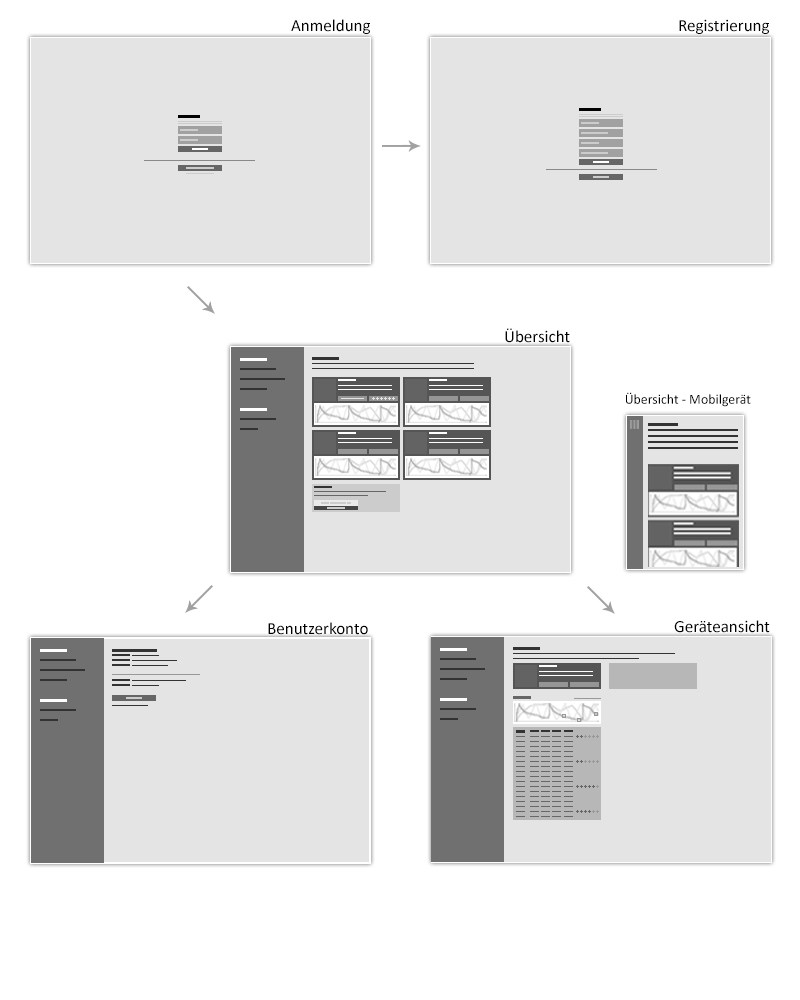
\includegraphics[width=1\textwidth]{images/wireframe-web.jpg}
  \caption{Greemon Konzept - Web Mockup}
  \label{fig:greemon-web-mockup}
\end{figure}

\begin{enumerate}
\item Anmelden: 
Vor der Benutzung der spezifischen Aufgaben muss das System dem Benutzer die Möglichkeit bieten sich anzumelden.

Bei der Registrierung und bei der Anmeldung soll das System eine bereits vorhandene, oder nicht bestätigte E-Mail Adresse erkennen können.

Angemeldet wird sich mit E-Mail Adresse und Passwort. Zum Anmelden werden diese Informationen in die vorgesehenen Felder eingetragen und die Schaltfläche „Anmelden“ betätigt. Ist kein Benutzer vorhanden, so steht die Schaltfläche „Registrieren“ zur Verfügung.

Um einen Benutzer zu Registrieren muss das System die Möglichkeit bieten einen neuen Benutzer anzulegen. Die E-Mail Adresse eines neu angelegten Benutzers muss bestätigt werden.

Wurde die Verbindung von Benutzername und Passwort nicht gefunden, soll das System dem Benutzer eine Fehlermeldung anzeigen. Hat der Benutzer sein Passwort vergessen muss ihm das System die Möglichkeit bieten sein Passwort ändern zu können. Wurde das Passwort zu einer E-Mail Adresse vergessen, so steht ein klickbarer Text „Passwort vergessen“ zur Verfügung. 


\item Registrieren: Erforderlich, wenn noch kein Benutzer vorhanden. Geräte werden einem Benutzer zugeordnet. Benötigte Informationen um einen Benutzer zu erstellen sind: E-Mail Adresse und Passwort. Beide Felder werden, um Tippfehler zu vermeiden doppelt abgefragt. Zugleich soll das Datum, so wie die Uhrzeit übermittelt und gespeichert werden. Das Passwort wird verschlüsselt abgelegt. Die E-Mail Adresse soll unverschlüsselt gespeichert werden. Die Seite wird verlassen mit erfolgreichem erstellen des Benutzers, oder mit einem Abbruch auf die Schaltfläche „Zurück“. Um einen Benutzer verwenden zu können ist es erforderlich die E-Mail Adresse zu bestätigen – Dazu wird beim Erstellen eine E-Mail an die angegebene Adresse gesendet, die der Benutzer bestätigen muss. 

\item Hauptmenü: Das ist der Startbildschirm nach dem Anmelden. Hier wird dem Benutzer eine Übersicht seiner registrierten Geräte, als „Steckbriefe“, gelistet. Ein Menü auf der linken Seite dient als Seiten-Navigation. Diese ist an die Größe des Bildschirmes angepasst. Der Inhalt der Seite beginnt mit dem Seitentitel „Übersicht“ unter dem ein kleiner Text die Funktion der Seite kurz erläutert. Darunter befinden sich die dem Benutzer zugeteilten Geräte. Ein „Steckbrief“ enthält die Informationen:
\begin{enumerate}
    \item Name des Gerätes.
    \item Bild der Pflanze, als „Symbol“.
    \item Letzte Aktivität (Letzte Nachricht erhalten) durch das Gerät.
    \item Eine durch den Benutzer eingegebene Beschreibung der Pflanze.
    \item Diagramm der letzten 24 Stunden mit der Anzeige der Bodenfeuchtigkeit.
    \item Klickbares Bewertungssystem. Diese Bewertung wird der zuletzt empfangenen Werteaufstellung zugeordnet und in der Datenbank gespeichert.
    \item Eine Schaltfläche um in die Detailansicht des Gerätes zu gelangen.
\end{enumerate}

Unter den „Steckbriefen“ ist ein Bereich um ein neues Gerät dem Benutzer zuzuordnen. Eine kurze Anleitung beschreibt dem Benutzer die Vorgehensweise. Ein Eingabefeld erlaubt die Eingabe des Registrierungsschlüssels. Dieser wurde bei der Initialisierung des Gerätes erstellt. Eine Schalfläche bestätigt die Eingabe. Das neue Gerät wird als neuer „Steckbrief“ unter den anderen Geräten angefügt. Sollte der Registrierungsschlüssel nicht gefunden werden können, so wird das dem Benutzer mitgeteilt.

Die Seitennavigation beinhaltet die Navigationsmöglichkeiten zu den Inhalten:
\begin{enumerate}
    \item Übersicht
    \item Einstellungen
    \item Abmelden 
\end{enumerate}

\item Einstellungen: Zeigt Benutzerinformationen an. Es ist möglich Informationen zu Ändern.
\begin{enumerate}
    \item E-Mail Adresse (Angezeigt, Änderbar). Änderung muss durch E-Mail bestätigt werden.
    \item Passwort (Nicht angezeigt, Änderbar). Der Benutzer wird bei einer Passwortänderung abgemeldet und muss sich erneut anmelden. Um das Passwort zu ändern wird aus Sicherheitsgründen das aktuelle Passwort benötigt.
    \item Registrierungsdatum und Uhrzeit (Angezeigt, Nicht änderbar).
    \item Anzahl registrierter Geräte (Angezeigt, Nicht änderbar). 
\end{enumerate}

\item Detailansicht: Diese Ansicht ändert den Inhalt der Seite auf Gerätespezifische Informationen. Angezeigt wird der „Steckbrief“ des Gerätes. Das Diagramm wird um weitere Anzeigen erweitert. Angezeigt werden nun: Luftfeuchtigkeit, Lichtintensität, Bodenfeuchtigkeit, Lichtintensität, Umgebungstemperatur, Qualität der Pflanze (Benutzereingabe). Die Werte können einzeln ein- und ausgeblendet werden.

Die Bewertung der Pflanze durch den Benutzer wird im Diagramm an dem entsprechenden Zeitpunkt als Balken angezeigt.

Hier kann der Benutzer auch einstellen ab welchem Schwellwert bei welchem Sensor eine E-Mail, als Information, gesendet werden soll. Diese werden nur gesendet, wenn die Option angeschaltet ist. Ist ein Schwellwert Min=Max eingestellt ist die Option automatisch für dieses Gerät abgeschalten.

\item Abmelden: Bringt den Benutzer zurück zur Anmeldeseite. Um die Inhalte der Applikation wieder benutzen zu können ist eine erneute Anmeldung erforderlich.

\item
Sonstiges: Wie in Abbildung \ref{fig:greemon-web-mockup} bei „Übersicht-Mobilgerät“ zu sehen, soll sich die Navigation bei einem mobilen Endgerät auf einen Balken beschränken und sich auf einen Klick auf das Menü-Symbol erweitern. Dies dient dazu den Platz auf der Anzeige platzsparend zu benutzen. 

\end{enumerate}





%%%%%%%%%%%%%%%%%%%%%%%%%%%%%%%%%%%%%%%%%%%%%%%%%%%%%%%%%%%%%%%%%%%%%%%%%%%%%%%%%%%%%
%
%
% Pflichtenheft Client
%
%
%%%%%%%%%%%%%%%%%%%%%%%%%%%%%%%%%%%%%%%%%%%%%%%%%%%%%%%%%%%%%%%%%%%%%%%%%%%%%%%%%%%%%

\newpage
\part{Pflichtenheft - Greemon Client}

\tableofcontents 

\newpage

\section{Zielbestimmung}
\subsection{Musskriterien}
        Ziel der Projektarbeit ist es ein Gerät zu entwickeln, dass die abiotischen Sensorwerte für eine Zimmerpflanze zyklisch auszulesen und an einen Server weiterzuleiten. Die zu beobachtenden Werte sind: Luftfeuchtigkeit, Bodenfeuchtigkeit, Lichtintensität, Umgebungstemperatur.
        Dazu werden die \textbf{Wertebereiche der Sensoren evaluiert} (Beinhaltet das Verifizieren der Funktionalität so wie das Untersuchen der im Datenblatt angegebenen Grenzwerte wie z.B. Datenrate und Genauigkeit). \textbf{Das Format der Datenübertragung zum Server} wird festgelegt. Die \textbf{Reichweite des CC3200 Chips, so wie die Verlustrate} ab bestimmten Distanzen und Umgebungen ermittelt. 
    Es wird eine Lösung zum \textbf{Speichern der Konfigurationsdatei} und zum temporären \textbf{Speichern gesammelter Sensorwerte} gesucht und implementiert. Das Gerät muss eine Möglichkeit besitzen Sensorwerte zu speichern, falls keine Verbindung zum Server besteht, um diese zu einem späteren Zeitpunkt zu übertragen.
\subsection{Wunschkriterien}
    Entwicklung einer Platine für eine Stromversorgung über eine Batterie. Sensor zum auslesen der CO2 Konzentration in der Luft. Konfiguration über eine Weboberfläche. Energie-Management für eine effizientere Akkulaufzeit.
\subsection{Abgrenzungskriterien}
    Eine Interpretation der gesammelten Daten erfolgt nicht durch den Mikrocontroller.
    Die Konfiguration des Mikrocontrollers umfasst nur zur Übertragung an den Server benötigte Daten.
    Das Gerät soll nicht im Außenbereich verwendet werden. Das Gehäuse wird nicht wasserdicht entworfen.
\section{Produkteinsatz}
\subsection{Anwendungsbereiche}
    Das Gerät wird bevorzugterweise in einem Gewächshaus, oder in geschlossenen Räumen verwendet. 
\subsection{Zielgruppen}
    Hobby-Gärtner, Benutzer ohne Programmiererfahrung. 
    %
    % TODO: Professor (Bewertet die Arbeit), Otto-Normalverbraucher
    %
\subsection{Bedingungen}
    Das Gerät wird nicht im Außenbereich benutzt. Eine Stromquelle steht zur Verfügung, wenn das Gerät ohne Batterie betrieben wird. Das WLAN-Netzwerk befindet sich in Reichweite.
\section{Produktumgebung}
\subsection{Software}
    Treiber zum emulieren eines virtuellen COM-Ports, so wie eine Software für die Ausgaben des Konfigurationsdialogs (bevorzugt Putty) müssen auf dem System installiert sein.
\subsection{Hardware}
    USB Port zum Anschluss des Gerätes, so wie ein Micro-USB-Kabel. Konfigurierter WLAN-Access-Point mit Internetverbindung. Eine zu beobachtende Zimmerpflanze.





%%%%%%%%%%%%%%%%%%%%%%%%%%%%%%%%%%%%%%%%%%%%%%%%%%%%%%%%%%%%%%%%%%%%%%%%%%%%%%
% USE-CASE Diagramme
%%%%%%%%%%%%%%%%%%%%%%%%%%%%%%%%%%%%%%%%%%%%%%%%%%%%%%%%%%%%%%%%%%%%%%%%%%%%%%
\section{Use-Case Diagramme}
\subsection{Allgemeines Use-Case Diagramm}
\begin{figure}[htbp] 
  \centering
     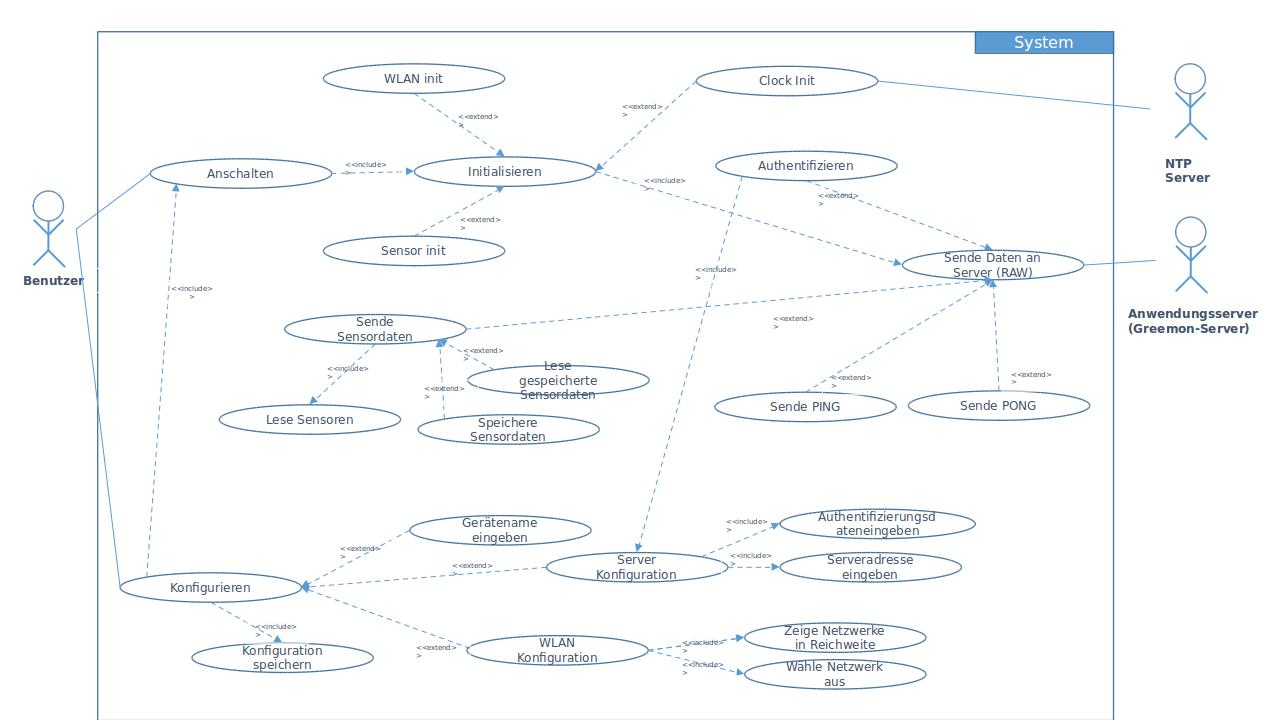
\includegraphics[width=1\textwidth]{images/usecase_client_allgemein.jpg}
  \caption{Greemon Client - Use-Case Allgemein}
  \label{fig:usecase_client_general}
\end{figure}

%%%%%%%%%%%%%%%%%%%%%%%%%%%%%%%%%%%%%%%%%%%%%%%%%%%%%%%%%%%%%%%%%%%%%%%%%%%%%%
% PRODUKTFUNKTIONEN
%%%%%%%%%%%%%%%%%%%%%%%%%%%%%%%%%%%%%%%%%%%%%%%%%%%%%%%%%%%%%%%%%%%%%%%%%%%%%%
\section{Produktfunktionen}

%%%%%%%%%%%%%%%%%%%%%%%%%%%%%%%%%%%%%%%%%%%%%%%%%%%%%%%%%%%%%%%%%%%%%%%%%%%%%%
% Grobentwurf des Systems
%%%%%%%%%%%%%%%%%%%%%%%%%%%%%%%%%%%%%%%%%%%%%%%%%%%%%%%%%%%%%%%%%%%%%%%%%%%%%%
\newpage
\subsection{Grobentwurf}

\begin{figure}[htbp] 
  \centering
     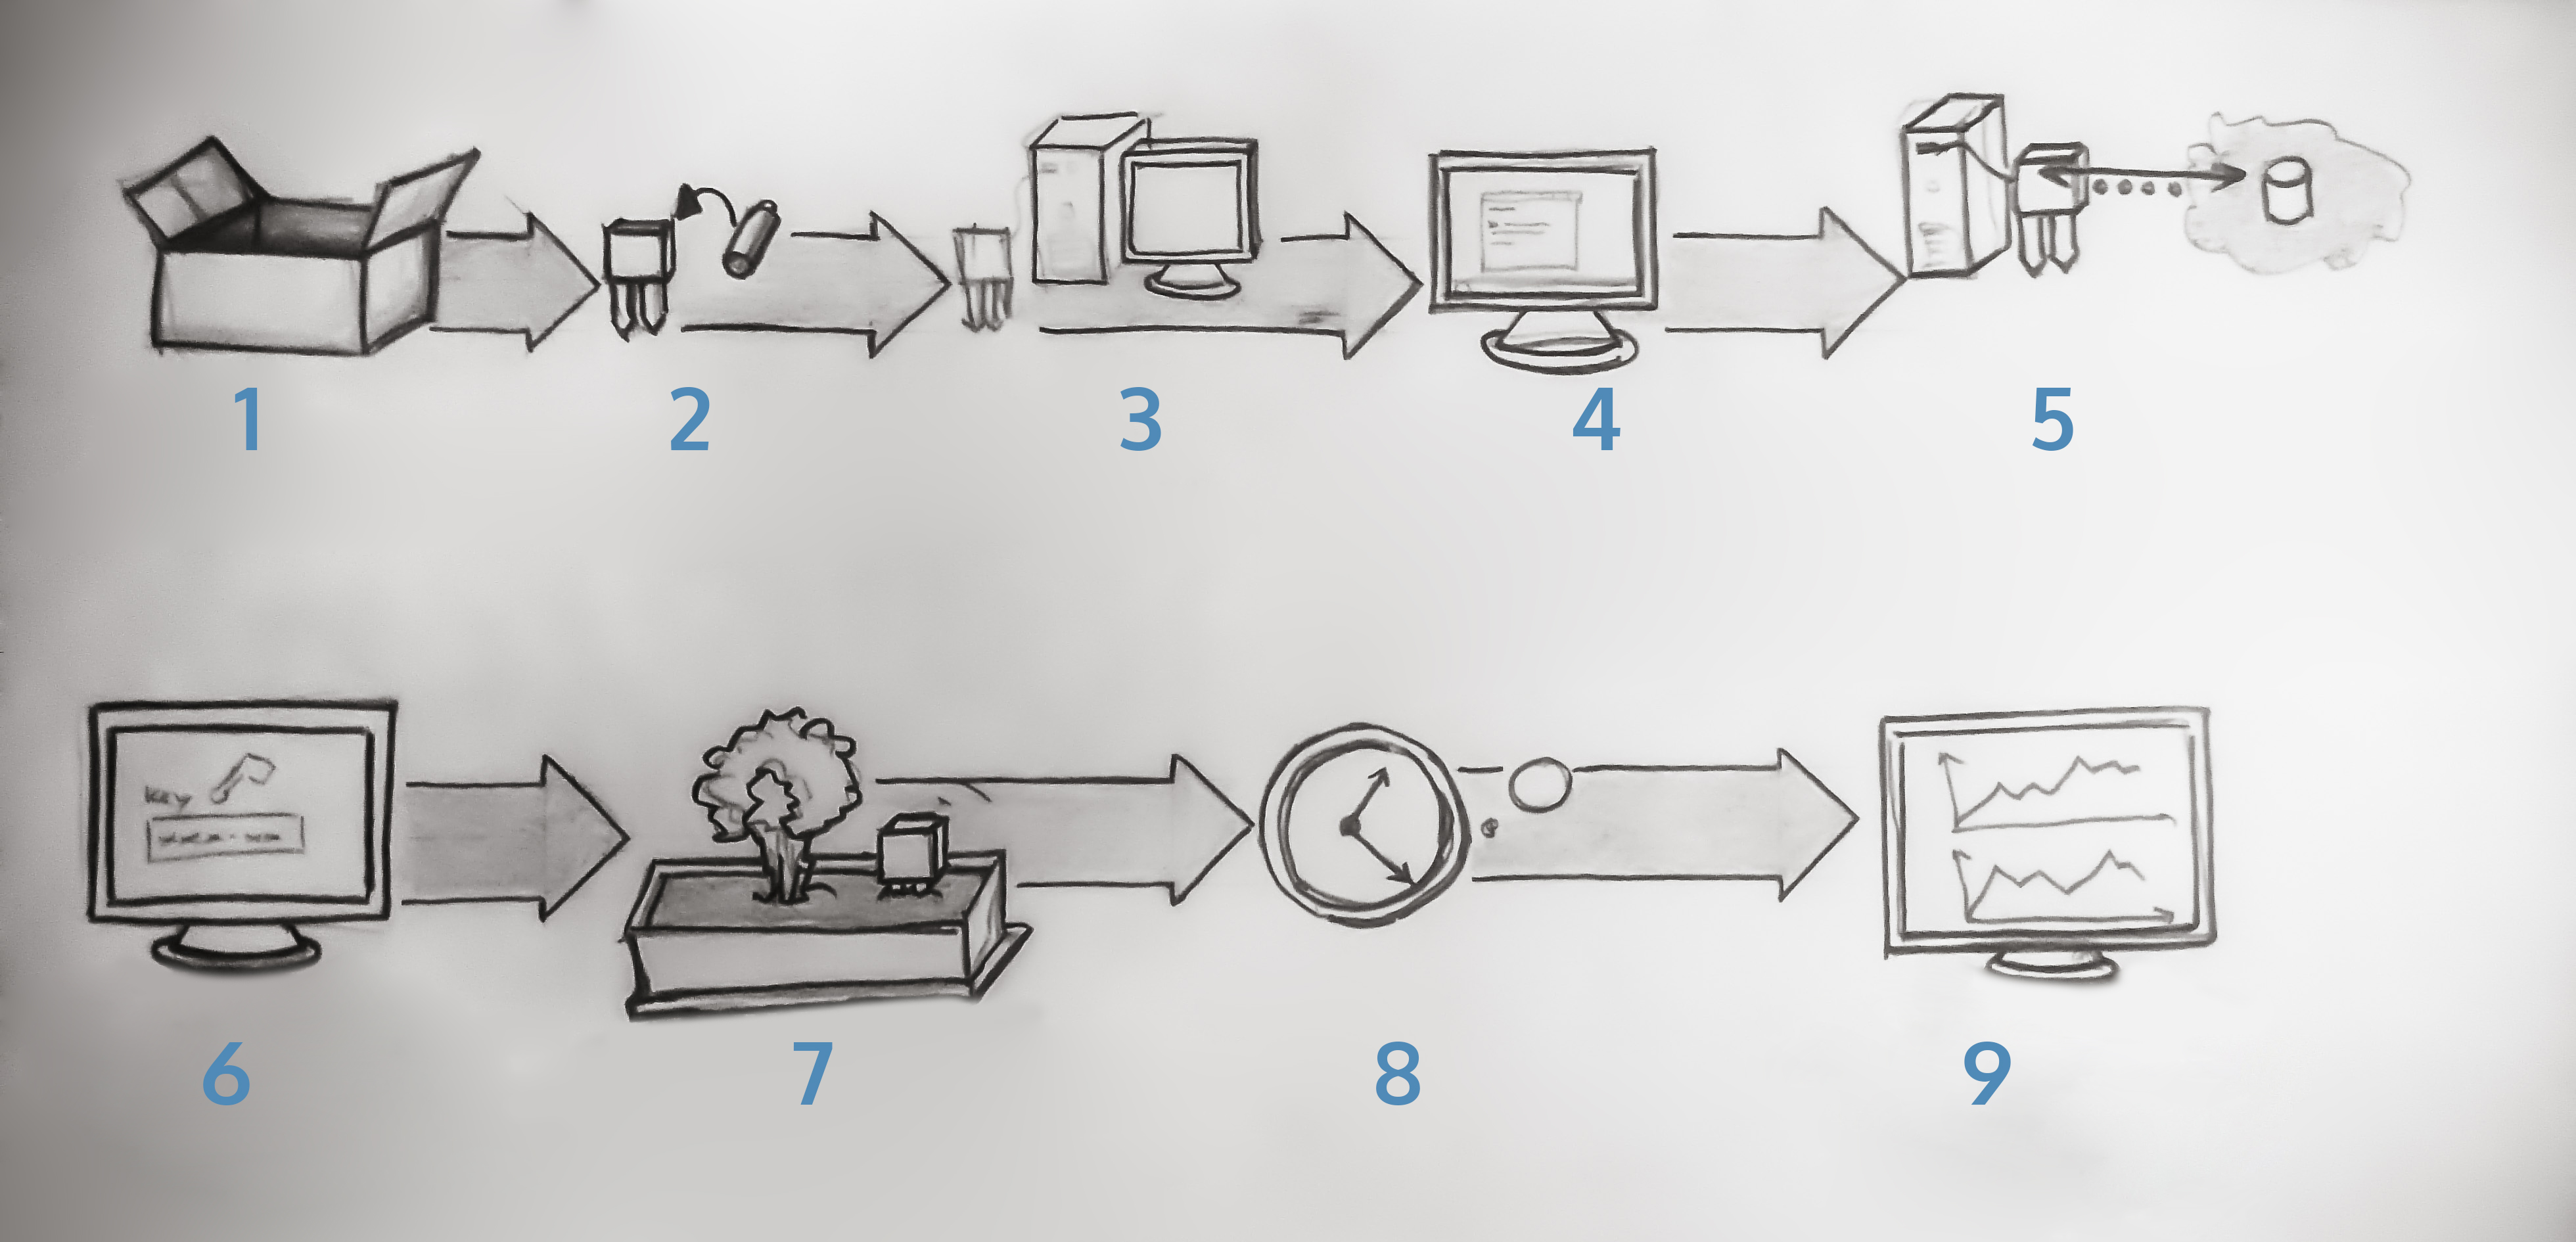
\includegraphics[width=1\textwidth]{images/Skizze_Quickstartguide_numeriert.jpg}
  \caption{Greemon Konzept - Client}
  \label{fig:Bild1}
\end{figure}

\begin{enumerate}
  
  \item Das erhaltene Gerät aus der Verpackung befreien 
  
  \item Einsetzen der Batterie oder 
  \begin{enumerate}
    \item  Eine auf dem Gerät befindliche rote LED indiziert den unkonfigurierten Status des Gerätes. Diese Leuchtet solange:
    \begin{enumerate}
      \item Keine Verbindung mit dem Server besteht oder 
      \item Keine Konfiguration vorliegt
    \end{enumerate}
  \end{enumerate}
  
  \item Verbinden mit der USB Schnittstelle des Computers 
    \begin{enumerate}
      \item Die Konfiguration des Gerätes erfolgt durch eine USB Verbindung, die durch einen virtuellen COM Port die Verbindung zum Gerät herstellt. 
    \end{enumerate}
    
  \item Konfigurieren 
  \begin{enumerate}
    \item Unterscheidung zwischen bereits konfiguriertem Gerät und einem neu zu konfigurierendem Gerät 
    \item Bei erster Verwendung 
        \begin{enumerate}
            \item Anzeige aller in Reichweite befindlichen WLAN Netzwerke mit Signalstärke und Verschlüsselungstyp 
            \item Auswahl des Netzwerkes und Eingabe des Passwortes 
            \item Eingabe der Server-Adresse 
            \item Anzeige des vom Server erhaltenen/generierten Registrierungsschlüssels. Dies erfordert eine Authentifizerung zum Server. Erst wenn die Daten korrekt sind, werdne die Daten übernommen.
        \end{enumerate}
    \item Bei bereits registriertem Gerät mit Verbindung zum Server 
        \begin{enumerate}
            \item Anzeige des Gerätenamens 
            \item Anzeige Registrierungsschlüssel 
            \item Anzeige Serveradresse 
            \item Anzeige WLAN Konfiguration und Signalstärke 
            \item Biete Löschung der Konfiguration an 
        \end{enumerate}  
    \item Bei bereits registriertem Gerät ohne Verbindung zum Server
        \begin{enumerate}
            \item Anzeige des Gerätenamens
            \item Anzeige Registrierungsschlüssel 
            \item Anzeige Serveradresse 
            \item Anzeige WLAN Konfiguration 
            \item Anzeige der letzten Verbindung und Internetstatus 
            \item Biete Löschung der Konfiguration an 
        \end{enumerate}        
    \end{enumerate}
        
    \item Verbindungsaufbau und Initialisierung
    \begin{enumerate}
        \item Verbindung mit dem Sever wird hergestellt. 
        \item Synchronisierung der Uhr mit einem NTP Server. 
        \item Anmeldung des Gerätes 
            \begin{enumerate}
                \item Die Identifikationsnummer des Gerätes wird übermittelt. 
                \item Ein Registrierungsschlüssel wird angezeigt             
            \end{enumerate}
    \end{enumerate}      
        
    \item Eingabe des Registrierungsschlüssels im Server-Webinterface    
    \begin{enumerate}
        \item Die Eingabe des Schlüssels dient zum logischen Verknüpfen des Gerätes mit einem Benutzerkonto.  
    \end{enumerate}
    
    \item Örtliche Platzierung des Gerätes in der Erde in der Nähe der Pflanze.  
    
    \item Sammeln von abiotischen Daten und Senden an den Server
    \begin{enumerate}
    \item Zyklische Übermittlung der gesammelten Werte. Auslesen von den Sensoren 
        \begin{enumerate}
        \item Bodenfeuchtigkeit (Muss)
        \item Luftfeuchtigkeit (Muss)
        \item CO2 Luft-Konzentration (Gewünscht)
        \item Lichtintensität (Muss)
        \item Umgebungstemperatur (Muss)
        \item Ladezustand der Batterie (Gewünscht)
        \end{enumerate}
    \item Anfügen der Werte an die der zu sendenden Werte 
    \item Senden der Werte-Sammlung an den Server und löschen der Werte bei erfolgreicher Übermittlung. Beinhaltet die Überprüfung einer Konnektivität zum Server. Dazu wird ein PING-Paket zum Server gesendet. Antwortet der Server mit einem Pong Packet, so können die Werte übermittelt werden.
    \end{enumerate}
    
    \item Anzeige der gesammelten Daten in der Web-Oberfläche.
  
\end{enumerate}

\subsection{Konzept des Aufbaus}
Siehe Abbildung \ref{fig:Bild1}, Nummer 7. Das Gerät steckt in der Erde der zu beobchtenden Pflanze.


\subsection{Funktionale Anforderungen}

\newcommand{\BreiteErsterTab}{3cm}
\newcommand{\BreiteZweiterTab}{10cm}




%%%%%%%%%%%%%%%%%%%%%%%%%%%%%%%%%%%%%%%%%%%%%%%%%%%%%%%%%%%%%%%%%%%%%%%%%%%%%%%%%%%%
% F000X Pre-Initialisierung
%%%%%%%%%%%%%%%%%%%%%%%%%%%%%%%%%%%%%%%%%%%%%%%%%%%%%%%%%%%%%%%%%%%%%%%%%%%%%%%%%%%%


\newcounter{req} 
\newcounter{reqGrp}[req] 
\newcounter{reqSub}[reqGrp] 
\newcounter{reqProc}[reqSub] 

\renewcommand\thereq{/F\arabic{req}000/} 
\renewcommand\thereqGrp{/F\arabic{req}\arabic{reqGrp}00/} 
\renewcommand\thereqSub{/F\arabic{req}\arabic{reqGrp}\arabic{reqSub}0/} 
\renewcommand\thereqProc{/F\arabic{req}\arabic{reqGrp}\arabic{reqSub}\arabic{reqProc}/} 




\newcommand{\requirement}[2]{% 
  \refstepcounter{req}
  \label{#1} 
  \thereq~#2
} 

\newcommand{\requirementGroup}[2]{% 
  \refstepcounter{reqGrp}
  \label{#1} 
  \thereqGrp~#2
} 

\newcommand{\requirementSubGroup}[2]{% 
  \refstepcounter{reqSub}
  \label{#1} 
  \thereqSub~#2
} 

\newcommand{\requirementProcess}[2]{% 
  \refstepcounter{reqProc}
  \label{#1} 
  \thereqProc~#2
} 

\newrefformat{req}{Anforderung \ref{#1}}


 %%%%%%%%%%%%%%%%%%%%%%%%%%%%%%%%%%%%%%%%%%%%%%%%%%%%%%%%%%%%%%%%%%%%%%%%%%%%%%%%%%%%
 % F1000 
 % Device startup
 % 
 %%%%%%%%%%%%%%%%%%%%%%%%%%%%%%%%%%%%%%%%%%%%%%%%%%%%%%%%%%%%%%%%%%%%%%%%%%%%%%%%%%%%

    
    \subsubsection{Inbetriebnahme}
    \begin{tabular}{|p{\BreiteErsterTab}|p{\BreiteZweiterTab}|}\hline
    Funktion-ID         & \requirement{req:greemon_startup}
                        \\ \hline
    Name                & Inbetriebnahme
                        \\ \hline
    Akteuere            & Benutzer
                        \\ \hline
    Ziel                & Das Gerät wird vom Benutzer in Betrieb genommen.
                        \\ \hline
    Einordnung          & Initialisierung 
                        \\ \hline
    Vorbedingungen      & Stromquelle angeschlossen 
                        \\ \hline
    Standardablauf      & Der Greemon startet automatisch, sobald eine Stromquelle angeschlossen wurde.
                        \\ \hline
    Nachbedingungen     & Startet den Initialisierungsprozess \ref{req:init_greemon}
                        \\ \hline
    Fehler              & Keine Stromquelle vorhanden.
                        \\ \hline
    Verzweigungen       & Keine 
                        \\ \hline
    Anmerkungen         & Keine 
                        \\ \hline
    Offene Fragen       & Keine
                        \\ \hline
 \end{tabular}
 
 
 %%%%%%%%%%%%%%%%%%%%%%%%%%%%%%%%%%%%%%%%%%%%%%%%%%%%%%%%%%%%%%%%%%%%%%%%%%%%%%%%%%%%
 % F011X 
 % Initialisierungen
 % 
 %%%%%%%%%%%%%%%%%%%%%%%%%%%%%%%%%%%%%%%%%%%%%%%%%%%%%%%%%%%%%%%%%%%%%%%%%%%%%%%%%%%%
 
 
 \subsubsection{Initialisierung Greemon}
 \begin{tabular}{|p{\BreiteErsterTab}|p{\BreiteZweiterTab}|}\hline
    Funktion-ID         &\requirementGroup{req:init_greemon}
                        \\ \hline
    Name                &   Initialisierung Greemon
                        \\ \hline
    Akteuere            &   NTP-Server, Greemon-Server
                        \\ \hline
    Ziel                &   Das Gerät ist konfigurierbar  
                            oder die Konfiguration wurde geladen. 
                            und Sensorwerte können an den Server übertragen werden. Der Interrupthandler wurde initialisiert.
                        \\ \hline
    Einordnung          &   Initialisierung 
                        \\ \hline
    Vorbedingungen      &   \ref{req:greemon_startup} Anschalten.
                            \ref{req:cfg} Konfiguration wurde durchgeführt.
                        \\ \hline
    Standardablauf      &   Starten von \ref{req:init_serial} Initialisierung der serien Schnittstelle.
                            Starten von \ref{req:init_wlan} Initialisierung WLAN, 
                            Starten von \ref{req:init_sensors} initialisierung Sensoren, 
                            Starten von \ref{req:init_clock} Initialisierung der internen Systemuhr.

                        \\ \hline
    Nachbedingungen     &  Alle Initialisierungen müssen erfolgreich abgeschlossen worden sein. Gerät kann sich dann am Server authentifizieren.
                            Die rote LED erlischt.
                        \\ \hline
    Fehler              &   WLAN konnte nicht initialisiert werden,
                            Es besteht keine Verbindung zum Internet,
                            Der NTP Server konnte nicht erreicht werden.
                        \\ \hline
    Verzweigungen       &   Überprüfung, ob das gerät bereits vom Benutzer konfiguriert wurde.
                        \\ \hline
    Anmerkungen         &   Eine rote LED indiziert den Status und erlischt, wenn das Gerät betriebsbereit ist. 
                        \\ \hline
    Offene Fragen       &   Keine
                        \\ \hline
 \end{tabular}
 
 
  \subsubsection{Initialisierung WLAN}
 \begin{tabular}{|p{\BreiteErsterTab}|p{\BreiteZweiterTab}|}\hline
   Funktion-ID          &\requirementSubGroup{req:init_wlan} 
                        \\ \hline
   Name                 & Initialisierung WLAN
                        \\ \hline
   Akteuere             & Greemon, Greemon-Server
                        \\ \hline
   Ziel                 & Das Gerät ist betriebsbereit. 
                        \\ \hline
    Einordnung          & Initialisierung 
                        \\ \hline
    Vorbedingungen      & \ref{req:init_greemon} Greemon-Initialisierung gestartet
                        \\ \hline
    Standardablauf      & Laden der WLAN Konfiguration. Verbinden mit dem WLAN Netzwerk.
                        \\ \hline
    Nachbedingungen     & Internetverbindung besteht. 
                        \\ \hline
    Fehler              & Es liegen keine Konfigurationsdaten für das WLAN-Netzwerk vor. 
                        \\ \hline
    Verzweigungen       & Keine 
                        \\ \hline
    Anmerkungen         & Keine 
                        \\ \hline
    Offene Fragen       & Welche Verschlüsselungsstandards sollen unterstützt werden (Offen, WEP, WPA, WPA2)?
                        \\ \hline
 \end{tabular} 
 
 
 \subsubsection{Initialisierung Sensoren}
 \begin{tabular}{|p{\BreiteErsterTab}|p{\BreiteZweiterTab}|}\hline
    Funktion-ID         &\requirementSubGroup{req:init_sensors} 
                        \\ \hline
    Name                &  Initialisierung Sensoren
                        \\ \hline
    Akteuere            & Greemon 
                        \\ \hline
    Ziel                & Das Gerät ist betriebsbereit. 
                        \\ \hline
    Einordnung          & Initialisierung 
                        \\ \hline
    Vorbedingungen      & \ref{req:init_greemon} Greemon-Initialisierung gestartet
                        \\ \hline
    Standardablauf      & /TODO
                        \\ \hline
    Nachbedingungen     &  Sensoren können gelesen werden. 
                        \\ \hline
    Fehler              & Keine 
                        \\ \hline
    Verzweigungen       & Keine 
                        \\ \hline
    Anmerkungen         & Keine 
                        \\ \hline
    Offene Fragen       & Können die Sensoren einfach ausgelesen werden, oder wird eine größere Routine (Wartezeiten,..) benötigt?
                        \\ \hline
 \end{tabular} 

 
 \subsubsection{Initialisierung Uhrzeit}
 \begin{tabular}{|p{\BreiteErsterTab}|p{\BreiteZweiterTab}|}\hline
    Funktion-ID         &\requirementSubGroup{req:init_clock}  
                        \\ \hline
    Name                & Initialisierung Uhrzeit
                        \\ \hline
    Akteuere            & Greemon, NTP-Server
                        \\ \hline
    Ziel                & Das Gerät hat die aktuellste Uhrzeit empfangen und aktualisiert diese durch einen internen Timer.
                        \\ \hline
    Einordnung          & Initialisierung 
                        \\ \hline
    Vorbedingungen      &   \ref{req:init_wlan} WLAN initialisiert.
                        \ref{req:init_greemon} Greemon-Initialisierung gestartet
                        \\ \hline
    Standardablauf      & Aktualisieren der Systemzeit durch NTP Server.
                        Initialisieren des internen Timers mit einem Interrupt Intervall von 5 Minuten.
                        \\ \hline
    Nachbedingungen     & Timer wird gestartet. Interne Systemzeit wird durch diesen internen Timer kontinuierlich aktualisiert.
                        \\ \hline
    Fehler              & Der Server konnte nicht erreicht werden. Der Server hat keine Uhrzeit geliefert. 
                        \\ \hline
    Verzweigungen       & Keine 
                        \\ \hline
    Anmerkungen         & Keine 
                        \\ \hline
    Offene Fragen       &  Welche NTP-Server Adresse wird verwendet?
                        \\ \hline
 \end{tabular} 
 
  \subsubsection{Initialisierung serielle Schnittstelle}
 \begin{tabular}{|p{\BreiteErsterTab}|p{\BreiteZweiterTab}|}\hline
    Funktion-ID         &  \requirementSubGroup{req:init_serial}  
                        \\ \hline
    Name                & Initialisierung Serielle Schnittstelle
                        \\ \hline
    Akteuere            & Greemon, Benutzer
                        \\ \hline
    Ziel                & Bereitstellen der Schnittstelle zum Konfigurieren des Gerätes.
                        \\ \hline
    Einordnung          & Konfiguration
                        \\ \hline
    Vorbedingungen      & \ref{req:init_greemon} Greemon-Initialisierung gestartet
                        \\ \hline
    Standardablauf      & 
                        \\ \hline
    Nachbedingungen     & Gerät ist betriebsbereit. Das Gerät kann konfiguriert werden.
                        \\ \hline
    Fehler              & Keine 
                        \\ \hline
    Verzweigungen       & Keine 
                        \\ \hline
    Anmerkungen         & Keine 
                        \\ \hline
    Offene Fragen       &  Welche Baudrate wird verwendet?
                        \\ \hline
 \end{tabular} 
 

%%%%%%%%%%%%%%%%%%%%%%%%%%%%%%%%%%%%%%%%%%%%%%%%%%%%%%%%%%%%%%%%%%%%%%%%%%%%%%%%%%%%
% F02XX 
% Konfiguration
% 
%%%%%%%%%%%%%%%%%%%%%%%%%%%%%%%%%%%%%%%%%%%%%%%%%%%%%%%%%%%%%%%%%%%%%%%%%%%%%%%%%%%% 
 
 \subsubsection{Konfiguration Greemon}
 \begin{tabular}{|p{\BreiteErsterTab}|p{\BreiteZweiterTab}|}\hline
    Funktion-ID         & \requirementGroup{req:cfg}
                        \\ \hline
    Name                & Konfiguration
                        \\ \hline
    Akteuere            & Greemon
                        \\ \hline
    Ziel                & Initialisierungswerte setzen. Konfigurationsoberfläche für den Benutzer bereitstellen. 
                        \\ \hline
    Einordnung          & Konfiguration 
                        \\ \hline
    Vorbedingungen      &  \ref{req:init_greemon} Gerät wurde initialisiert. 
                        \ref{req:init_serial} Serielle Schnittstelle wurde initialisiert.
                        \\ \hline
    Standardablauf      &   Greemon wird via USB an einen Computer angeschlossen. 
                            Eine Verbindung wird über eine virtuelle serielle Schnittstelle aufgebaut. 
                            Der Benutzer öffnet ein Programm (Putty) und trägt die Baudrate, so wie den COM Port ein.
                            Das Gerät antwortet mit einem geführten Konfigurationsdialog. 
                            Der Benutzer bestätigt die Speicherung und erhält einen Registrierungsschlüssel. 
                            (Wird benötigt um das Gerät mit dem Greemon-Server Benutzer zu Verknüpfen)
                        \\ \hline
    Nachbedingungen     & Gerät wurde konfiguriert. Eine Internetverbindung besteht. Am Server authentifiziert. Registrierungsschlüssel erhalten.
                        \ref{req:cfg_save} wird zum Speichern der Daten ausgeführt.
                        \\ \hline
    Fehler              & Keine 
                        \\ \hline
    Verzweigungen       & Keine 
                        \\ \hline
    Anmerkungen         & Keine 
                        \\ \hline
    Offene Fragen       & Keine
                        \\ \hline
 \end{tabular} 
 
 
  \subsubsection{Konfiguration speichern}
 \begin{tabular}{|p{\BreiteErsterTab}|p{\BreiteZweiterTab}|}\hline
    Funktion-ID         & \requirementProcess{req:cfg_save} 
                        \\ \hline
    Name                &   Konfiguration
                        \\ \hline
    Akteuere            &   Greemon
                        \\ \hline
    Ziel                &   Initialisierungswerte setzen. Speichert die Daten persistent. 
                        \\ \hline
    Einordnung          &   Konfiguration 
                        \\ \hline
    Vorbedingungen      &   Erfolgreiche Ausführung von \ref{req:cfg} Konfiguration Greemon.
                        \\ \hline
    Standardablauf      &  Zeige den durch den Server generierten Registrierungsschlüssel an.
                        \\ \hline
    Nachbedingungen     &   Gerät ist betriebsbereit.
                        \\ \hline
    Fehler              &   Keine 
                        \\ \hline
    Verzweigungen       &   Keine 
                        \\ \hline
    Anmerkungen         &   Keine 
                        \\ \hline
    Offene Fragen       &   Wie können die Daten persistent gespeichert werden? 
                            Wie viel Speicherplatz ist auf dem Gerät verfügbar?
                        \\ \hline
 \end{tabular}
 
 
 \subsubsection{Konfiguration Gerätename}
 \begin{tabular}{|p{\BreiteErsterTab}|p{\BreiteZweiterTab}|}\hline
    Funktion-ID         & \requirementProcess{req:cfg_setDeviceName} 
                        \\ \hline
    Name                &  Konfiguration Gerätename            
                        \\ \hline
    Akteuere            & Greemon, Benutzer
                        \\ \hline
    Ziel                &  Der Benutzer hat dem Gerät einen Namen gegeben. Der Name wurde gespeichert.           
                        \\ \hline
    Einordnung          &  Konfiguration      
                        \\ \hline
    Vorbedingungen      &  \ref{req:init_serial} Serielle Schnittstelle wurde initialisiert.
                           \ref{req:cfg} Benutzer befindet sich im Konfigurationsdialog. 
                        \\ \hline
    Standardablauf      &  Eingabe des Namens über eine Consolenanwendung. Bestätigung durch Enter-Taste.  
                        \\ \hline
    Nachbedingungen     &   Eingabe Korrekt, ansonsten starte diesen Prozess neu und gebe dem Benutzer eine Fehlermeldung.
                        \\ \hline
    Fehler              &  Eingabe entspricht der erwarteten Form.    
                        \\ \hline
    Verzweigungen       &     
                        \\ \hline
    Anmerkungen         &  
                        \\ \hline
    Offene Fragen       &  Wie viele Zeichen darf der Name enthalten? Welche Zeichen dürfen enthalten sein?
                        \\ \hline
 \end{tabular}  
 
 
 \subsubsection{Konfiguration WLAN}
 \begin{tabular}{|p{\BreiteErsterTab}|p{\BreiteZweiterTab}|}\hline
    Funktion-ID         & \requirementSubGroup{req:cfg_setWLAN} 
                        \\ \hline
    Name                &  Konfiguration WLAN            
                        \\ \hline
    Akteuere            & Greemon, Benutzer
                        \\ \hline
    Ziel                &  Eine Verbindung zum Internet herstellen.
                        \\ \hline
    Einordnung          &  Konfiguration      
                        \\ \hline
    Vorbedingungen      &   \ref{req:init_serial} Serielle Schnittstelle wurde initialisiert.
                            \ref{req:cfg} Benutzer befindet sich im Konfigurationsdialog. 
                            \ref{req:cfg_setDeviceName} Gerätename wurde eingetragen.  
                        \\ \hline
    Standardablauf      &   Überprüfung der eingegebenen Daten. 
                            Verbinde mit dem WLAN Netzwerk.
                        \\ \hline
    Nachbedingungen     &  Eine Internetverbindung besteht.
                        \\ \hline
    Fehler              &  Eingegebene Authentifizierungsdaten sind nicht gültig.
                            WLAN Netzwerk ohne Internetverbindung.
                        \\ \hline
    Verzweigungen       &   Besteht eine Internetverbingung, weiter zu \ref{req:cfg_Server} Serverkonfiguration.
                            Besteht keine Internetverbindung wird die Konfiguration vom Benutzer erneut gefordert.   
                        \\ \hline
    Anmerkungen         &   -    
                        \\ \hline
    Offene Fragen       &  Welche Adresse soll zur Überprüfung einer bestehenden Internetverbindung erreicht werden können?   
                        \\ \hline
 \end{tabular} 
 
 
 \subsubsection{Konfiguration WLAN : Zeige Netzwerke in Reichweite}
 \begin{tabular}{|p{\BreiteErsterTab}|p{\BreiteZweiterTab}|}\hline
    Funktion-ID         & \requirementSubGroup{req:cfg_showNetwork}   
                        \\ \hline
    Name                &  Zeige WLAN Netzwerke in Reichweite            
                        \\ \hline
    Akteuere            & Greemon, Benutzer
                        \\ \hline
    Ziel                &  Ausgabe einer Liste mit verfügbaren WLAN Netzwerken.           
                        \\ \hline
    Einordnung          &  Konfiguration       
                        \\ \hline
    Vorbedingungen      &   Gestartet durch \ref{req:cfg_setWLAN} Konfiguration WLAN
                        \\ \hline
    Standardablauf      &  Dem Benutzer werden alle in Reichweite befindlichen WLAN Netzwerke 
                            mit Signalstärke und Verschlüsselungsart angezeigt.   
                        \\ \hline
    Nachbedingungen     &  Benutzer wählt ein Netzwerk aus \ref{req:cfg_setNetwork}.
                        \\ \hline
    Fehler              &  Es können keine WLAN Netzwerke gefunden werden.     
                        \\ \hline
    Verzweigungen       &  Aktualisieren. Der Prozess wird neu ausgeführt.   
                        \\ \hline
    Anmerkungen         &       
                        \\ \hline
    Offene Fragen       &     
                        \\ \hline
 \end{tabular} 
 

 \subsubsection{Konfiguration WLAN : Netzwerk auswählen}
 \begin{tabular}{|p{\BreiteErsterTab}|p{\BreiteZweiterTab}|}\hline
    Funktion-ID         & \requirementSubGroup{req:cfg_setNetwork}  
                        \\ \hline
    Name                &  WLAN Netzwerk auswählen            
                        \\ \hline
    Akteuere            & Greemon, Benutzer
                        \\ \hline
    Ziel                &  Authetifizierungsdaten wurden dem Gerät übergeben.           
                        \\ \hline
    Einordnung          &  Konfiguration      
                        \\ \hline
    Vorbedingungen      &  Benutzer hat im Prozess \ref{req:cfg_showNetwork} (Zeige Netzwerkliste) eine gültige Nummer für ein WLAN Netzwerk ausgewählt. 
                            Die Daten des ausgewählten Netzwerkes wurden an den Prozess weitergegeben. Das ist mindestens die SSID.
                        \\ \hline
    Standardablauf      &  Überspringe den Prozess, wenn das WLAN-Netzwerk keine Authentifizierung benötigt.
                            Benutzer trägt zu dem ausgewählten Prozess das Passwort des WLAN Netzwerkes ein.
                        \\ \hline
    Nachbedingungen     &  Teste Internetverbindung
                            Gebe E_NOCONN (<0) zurück wenn keine Verbindung besteht. SUCCESS (0) bei erfolgreicher Internetverbindung.
                        \\ \hline
    Fehler              &  -      
                        \\ \hline
    Verzweigungen       &  -   
                        \\ \hline
    Anmerkungen         &  -    
                        \\ \hline
    Offene Fragen       &  - 
                        \\ \hline
 \end{tabular} 
 
 \subsubsection{Konfiguration Greemon-Server}
 \begin{tabular}{|p{\BreiteErsterTab}|p{\BreiteZweiterTab}|}\hline
    Funktion-ID         & \requirementSubGroup{req:cfg_Server}  
                        \\ \hline
    Name                &  Konfiguration Greemon-Server Verbindungsdaten             
                        \\ \hline
    Akteuere            &  Greemon, Benutzer
                        \\ \hline
    Ziel                &  Die Adresse und der Port unter dem der Server erreichbar ist werden hinterlegt.           
                        \\ \hline
    Einordnung          &  Konfiguration     
                        \\ \hline
    Vorbedingungen      &  Benutzer hält die Daten zur Eingabe bereit. Die Verbindung mit dem Internet wurde in \ref{req:cfg_setWLAN} Konfiguration WLAN hergestellt.
                        \\ \hline
    Standardablauf      &  Aufruf des Dialogs zur Eingabe der Serverdaten \ref{req:cfg_setServerAddress}.  
                           Aufruf des Diaglogs zur Eingabe der Authentifizierungsdaten \ref{req:cfg_setServerLogin}.  
                           
                        Die in den Dialogen eingegebenen Daten werden überprüft. Je nach Fehler wird der Benutzer zurück zu dem jeweiligen Konfigurationsdialog geführt.
                        \\ \hline
    Nachbedingungen     &   
                        \\ \hline
    Fehler              &  
                            \begin{itemize}
                            \item E\_NOSERVER: Keine Verbindung zum Server wegen falschen Daten. 
                            \item E\_NOCONN: Keine Verbindung zum Server, keine Internetverbindung. 
                            \item E\_NOAUTH: Falsche Authentifizierungsdaten.
                            \end{itemize}
                        \\ \hline
    Verzweigungen       &  Bei E\_NOSERVER wird Dialog \ref{req:cfg_setServerAddress} wieder aufgerufen.
                            Bei E\_NOCONN wird Dialog \ref{req:cfg_setWLAN} wieder aufgerufen.
                            Bei E\_NOAUTH wird Dialog \ref{req:cfg_setServerLogin} wieder aufgerufen.
                        \\ \hline
    Anmerkungen         &  -
                        \\ \hline
    Offene Fragen       &  Nur IP oder auch Domain erlaubt?   
                        \\ \hline
 \end{tabular} 


 \subsubsection{Konfiguration Serververbindung : Serverdaten}
 \begin{tabular}{|p{\BreiteErsterTab}|p{\BreiteZweiterTab}|}\hline
    Funktion-ID         & \requirementSubGroup{req:cfg_setServerAddress} 
                        \\ \hline
    Name                &              
                        \\ \hline
    Akteuere            & Greemon, Benutzer
                        \\ \hline
    Ziel                &             
                        \\ \hline
    Einordnung          &  Konfiguration      
                        \\ \hline
    Vorbedingungen      &    
                        \\ \hline
    Standardablauf      &  Im Dialog wird der Benutzer aufgeforder die Adresse, so wie den Port des Servers anzugeben.  
                        \\ \hline
    Nachbedingungen     &   
                        \\ \hline
    Fehler              &       
                        \\ \hline
    Verzweigungen       &     
                        \\ \hline
    Anmerkungen         &       
                        \\ \hline
    Offene Fragen       &     
                        \\ \hline
 \end{tabular} 
 
 
 \subsubsection{Konfiguration Serververbindung : Authentifizierungsdaten}
 \begin{tabular}{|p{\BreiteErsterTab}|p{\BreiteZweiterTab}|}\hline
    Funktion-ID         & \requirementSubGroup{req:cfg_setServerLogin}   
                        \\ \hline
    Name                &              
                        \\ \hline
    Akteuere            & Greemon, Benutzer
                        \\ \hline
    Ziel                &             
                        \\ \hline
    Einordnung          &  Konfiguration      
                        \\ \hline
    Vorbedingungen      &    
                        \\ \hline
    Standardablauf      &  Im Dialog wird der Benutzer aufgefordert den Benutzernamen / E-Mail Adresse und sein Passwort für den Server einzugeben.
                        \\ \hline
    Nachbedingungen     &  Eingaben entsprechen der erwarteten Norm. Für E-Mail gilt: Es muss enthalten sein: Ein @-Zeichen, so wie mindestens ein .
                        \\ \hline
    Fehler              &       
                        \\ \hline
    Verzweigungen       &     
                        \\ \hline
    Anmerkungen         &       
                        \\ \hline
    Offene Fragen       &     
                        \\ \hline
 \end{tabular} 

%%%%%%%%%%%%%%%%%%%%%%%%%%%%%%%%%%%%%%%%%%%%%%%%%%%%%%%%%%%%%%%%%%%%%%%%%%%%%%%%%%%%
% F03XX 
% Server Konnektivität
% 
%%%%%%%%%%%%%%%%%%%%%%%%%%%%%%%%%%%%%%%%%%%%%%%%%%%%%%%%%%%%%%%%%%%%%%%%%%%%%%%%%%%%

 \subsubsection{Konnektivität zum Server}
 \begin{tabular}{|p{\BreiteErsterTab}|p{\BreiteZweiterTab}|}\hline
   Funktion-ID          & \requirementGroup{req:conn}  
                        \\ \hline
   Name                 & Serververbindung
                        \\ \hline
   Akteuere             & Greemon, Greemon-Server\\ \hline
   Ziel                 & 
                        \\ \hline
    Einordnung          & Server-Verbindung 
                        \\ \hline
    Vorbedingungen      &  
                        \\ \hline
    Standardablauf      & 
                        \\ \hline
    Nachbedingungen     & 
                        \\ \hline
    Fehler              & Keine 
                        \\ \hline
    Verzweigungen       & Keine 
                        \\ \hline
    Anmerkungen         & Keine 
                        \\ \hline
    Offene Fragen       & Keine
                        \\ \hline
 \end{tabular} 

 \subsubsection{Serverbindung erstellen}
 \begin{tabular}{|p{\BreiteErsterTab}|p{\BreiteZweiterTab}|}\hline
   Funktion-ID          & \requirementSubGroup{req:conn_create}  
                        \\ \hline
   Name                 & Verbindung zum Greemon-Server herstellen
                        \\ \hline
   Akteuere             & Greemon, Greemon-Server
                        \\ \hline
   Ziel                 & Die Verbindung zum Server wurde initialisiert. 
                        \\ \hline
    Einordnung          & Server-Verbindung
                        \\ \hline
    Vorbedingungen      & 
                        \\ \hline
    Standardablauf      &
                        \\ \hline
    Nachbedingungen     & 
                        \\ \hline
    Fehler              & Keine 
                        \\ \hline
    Verzweigungen       & 
                        \\ \hline
    Anmerkungen         & 
                        \\ \hline
    Offene Fragen       &
                        \\ \hline
 \end{tabular} 
 
 \subsubsection{/F0302/ - Authentifizierung am Greemon-Server}
 \begin{tabular}{|p{\BreiteErsterTab}|p{\BreiteZweiterTab}|}\hline
    Funktion-ID &        /F0302/  
                        \\ \hline
    Name &               Authentifizierung am Greemon-Server
                        \\ \hline
    Akteuere &           Greemon, Greemon-Server
                        \\ \hline
    Ziel &               Das Gerät ist betriebsbereit. 
                        \\ \hline
    Einordnung &        Server-Verbindung
                        \\ \hline
    Vorbedingungen &    Gerät wurde bereits durch den Benutzer konfiguriert.
                        WLAN Initialisiert.
                        \\ \hline
    Standardablauf &    
                        \\ \hline
    Nachbedingungen &   
                        \\ \hline
    Fehler &            Es besteht keine Verbindung zum Server 
                        Das Passwort oder der Benutzername sind falsch
                        \\ \hline
    Verzweigungen &     
                        \\ \hline
    Anmerkungen &       
                        \\ \hline
    Offene Fragen &     
                        \\ \hline
 \end{tabular} 
 
 \subsubsection{/F0310/ - Sende Daten RAW}
 \begin{tabular}{|p{\BreiteErsterTab}|p{\BreiteZweiterTab}|}\hline
    Funktion-ID &       /F0310/  
                        \\ \hline
    Name &              Sende Daten RAW
                        \\ \hline
    Akteuere &          Greemon, Greemon-Server
                        \\ \hline
    Ziel &              Senden von unbestimmten Daten an den Server. 
                        \\ \hline
    Einordnung &        Server-Verbindung
                        \\ \hline
    Vorbedingungen &    Sendepuffer ist mit Daten gefüllt
                        \\ \hline
    Standardablauf &    
                        \\ \hline
    Nachbedingungen &   
                        \\ \hline
    Fehler &       
                        \\ \hline
    Verzweigungen &     
                        \\ \hline
    Anmerkungen &       
                        \\ \hline
    Offene Fragen &     
                        \\ \hline
 \end{tabular} 
 
 \subsubsection{/F0311/ - Sende Daten PING}
 \begin{tabular}{|p{\BreiteErsterTab}|p{\BreiteZweiterTab}|}\hline
   Funktion-ID          & /F0311/  
                        \\ \hline
   Name                 & Sende Daten PING
                        \\ \hline
   Akteuere             & Greemon, Greemon-Server
                        \\ \hline
   Ziel                 & Senden von einem Ping Packet an den Server 
                        \\ \hline
    Einordnung          &  Server-Verbindung 
                        \\ \hline
    Vorbedingungen      &   
                        \\ \hline
    Standardablauf      &  
                        \\ \hline
    Nachbedingungen     &   
                        \\ \hline
    Fehler              & Server antwortet nicht auf Ping-Anfrage. 
                        \\ \hline
    Verzweigungen       &   
                        \\ \hline
    Anmerkungen         &   
                        \\ \hline
    Offene Fragen       &   
                        \\ \hline
 \end{tabular} 
 
 \subsubsection{/F0312/ - Sende Daten PONG}
 \begin{tabular}{|p{\BreiteErsterTab}|p{\BreiteZweiterTab}|}\hline
   Funktion-ID          & /F0312/  
                        \\ \hline
   Name                 & Sende Daten PONG
                        \\ \hline
   Akteuere             & Greemon, Greemon-Server
                        \\ \hline
   Ziel                 & Antwort zu einem Ping Packet senden 
                        \\ \hline
    Einordnung          &  Server-Verbindung 
                        \\ \hline
    Vorbedingungen      & 
                        \\ \hline
    Standardablauf      & 
                        \\ \hline
    Nachbedingungen     &  
                        \\ \hline
    Fehler              & Keine 
                        \\ \hline
    Verzweigungen       & 
                        \\ \hline
    Anmerkungen         &  
                        \\ \hline
    Offene Fragen       & 
                        \\ \hline
 \end{tabular} 

 \subsubsection{/F0313/ - Sende Daten Sensoren}
 \begin{tabular}{|p{\BreiteErsterTab}|p{\BreiteZweiterTab}|}\hline
   Funktion-ID          & /F0313/  
                        \\ \hline
   Name                 & Sende Sensordaten
                        \\ \hline
   Akteuere             & Greemon, Greemon-Server
                        \\ \hline
   Ziel                 & Starte die Ausleseprozesse. 
                            Speichere Daten. 
                            Sende gesammelte Daten an den Server. 
                            Lösche gesendete Daten. 
                        \\ \hline
    Einordnung          &  Server-Verbindung 
                        \\ \hline
    Vorbedingungen      &  
                        \\ \hline
    Standardablauf      & 
                        \\ \hline
    Nachbedingungen     &  
                        \\ \hline
    Fehler              & Keine 
                        \\ \hline
    Verzweigungen       &  
                        \\ \hline
    Anmerkungen         &  
                        \\ \hline
    Offene Fragen       & 
                        \\ \hline
 \end{tabular} 


%%%%%%%%%%%%%%%%%%%%%%%%%%%%%%%%%%%%%%%%%%%%%%%%%%%%%%%%%%%%%%%%%%%%%%%%%%%%%%%%%%%% 
% F04XX 
% Storage Sensordata - Read and Write
%
%%%%%%%%%%%%%%%%%%%%%%%%%%%%%%%%%%%%%%%%%%%%%%%%%%%%%%%%%%%%%%%%%%%%%%%%%%%%%%%%%%%%

 \subsubsection{/F0410/ - Lese Sensoren}
 \begin{tabular}{|p{\BreiteErsterTab}|p{\BreiteZweiterTab}|}\hline
    Funktion-ID &       /F0411/  
                        \\ \hline
    Name &              Lese Sensoren
                        \\ \hline
    Akteuere &          Greemon
                        \\ \hline
    Ziel &              Gibt eine Struktur mit den gelesenen Sensorwerten zurück.
                        \\ \hline
    Einordnung &        
                        \\ \hline
    Vorbedingungen &    
                        \\ \hline
    Standardablauf &    
                        \\ \hline
    Nachbedingungen &   
                        \\ \hline
    Fehler &       
                        \\ \hline
    Verzweigungen &     
                        \\ \hline
    Anmerkungen &       
                        \\ \hline
    Offene Fragen &     
                        \\ \hline
 \end{tabular} 

 \subsubsection{/F0411/ - Lese Sensor Bodenfeuchtigkeit}
 \begin{tabular}{|p{\BreiteErsterTab}|p{\BreiteZweiterTab}|}\hline
    Funktion-ID &       /F0411/  
                        \\ \hline
    Name &              Lese Sensor Bodenfeuchtigkeit
                        \\ \hline
    Akteuere &          Greemon
                        \\ \hline
    Ziel &             
                        \\ \hline
    Einordnung &        
                        \\ \hline
    Vorbedingungen &    
                        \\ \hline
    Standardablauf &    
                        \\ \hline
    Nachbedingungen &   
                        \\ \hline
    Fehler &       
                        \\ \hline
    Verzweigungen &     
                        \\ \hline
    Anmerkungen &       
                        \\ \hline
    Offene Fragen &     
                        \\ \hline
 \end{tabular} 

 \subsubsection{/F0412/ - Lese Sensor Luftfeuchtigkeit}
 \begin{tabular}{|p{\BreiteErsterTab}|p{\BreiteZweiterTab}|}\hline
    Funktion-ID &       /F0412/  
                        \\ \hline
    Name &              Lese Sensor Luftfeuchtigkeit
                        \\ \hline
    Akteuere &          Greemon
                        \\ \hline
    Ziel &             
                        \\ \hline
    Einordnung &        
                        \\ \hline
    Vorbedingungen &    
                        \\ \hline
    Standardablauf &    
                        \\ \hline
    Nachbedingungen &   
                        \\ \hline
    Fehler &       
                        \\ \hline
    Verzweigungen &     
                        \\ \hline
    Anmerkungen &       
                        \\ \hline
    Offene Fragen &     
                        \\ \hline
 \end{tabular} 
 
 \subsubsection{/F0413/ - Lese Sensor Temperatur}
 \begin{tabular}{|p{\BreiteErsterTab}|p{\BreiteZweiterTab}|}\hline
    Funktion-ID &       /F0413/  
                        \\ \hline
    Name &              Lese Sensor Temperatur
                        \\ \hline
    Akteuere &          Greemon
                        \\ \hline
    Ziel &             
                        \\ \hline
    Einordnung &        
                        \\ \hline
    Vorbedingungen &    
                        \\ \hline
    Standardablauf &    
                        \\ \hline
    Nachbedingungen &   
                        \\ \hline
    Fehler &       
                        \\ \hline
    Verzweigungen &     
                        \\ \hline
    Anmerkungen &       
                        \\ \hline
    Offene Fragen &     
                        \\ \hline
 \end{tabular} 
 
 \subsubsection{/F0414/ - Lese Sensor Licht}
 \begin{tabular}{|p{\BreiteErsterTab}|p{\BreiteZweiterTab}|}\hline
    Funktion-ID &       /F0414/  
                        \\ \hline
    Name &              Lese Sensor Licht
                        \\ \hline
    Akteuere &          Greemon
                        \\ \hline
    Ziel &             
                        \\ \hline
    Einordnung &        
                        \\ \hline
    Vorbedingungen &    
                        \\ \hline
    Standardablauf &    
                        \\ \hline
    Nachbedingungen &   
                        \\ \hline
    Fehler &       
                        \\ \hline
    Verzweigungen &     
                        \\ \hline
    Anmerkungen &       
                        \\ \hline
    Offene Fragen &     
                        \\ \hline
 \end{tabular} 
 
 \subsubsection{/F0500/ - Sensorspeicher Initialisieren}
 \begin{tabular}{|p{\BreiteErsterTab}|p{\BreiteZweiterTab}|}\hline
    Funktion-ID &       /F0500/  
                        \\ \hline
    Name &              Speicher Speichern Sensordaten
                        \\ \hline
    Akteuere &          Greemon
                        \\ \hline
    Ziel &             
                        \\ \hline
    Einordnung &        
                        \\ \hline
    Vorbedingungen &    
                        \\ \hline
    Standardablauf &    
                        \\ \hline
    Nachbedingungen &   
                        \\ \hline
    Fehler &       
                        \\ \hline
    Verzweigungen &     
                        \\ \hline
    Anmerkungen &       
                        \\ \hline
    Offene Fragen &     
                        \\ \hline
 \end{tabular}  
 
 \subsubsection{/F0510/ - Sensorspeicher Sensordaten speichern}
 \begin{tabular}{|p{\BreiteErsterTab}|p{\BreiteZweiterTab}|}\hline
    Funktion-ID &       /F0500/  
                        \\ \hline
    Name &              Speicher Speichern Sensordaten
                        \\ \hline
    Akteuere &          Greemon
                        \\ \hline
    Ziel &             
                        \\ \hline
    Einordnung &        
                        \\ \hline
    Vorbedingungen &    
                        \\ \hline
    Standardablauf &    
                        \\ \hline
    Nachbedingungen &   
                        \\ \hline
    Fehler &       
                        \\ \hline
    Verzweigungen &     
                        \\ \hline
    Anmerkungen &       
                        \\ \hline
    Offene Fragen &     
                        \\ \hline
 \end{tabular} 
 
 \subsubsection{/F0520/ - Sensorspeicher Sensordaten lesen }
 \begin{tabular}{|p{\BreiteErsterTab}|p{\BreiteZweiterTab}|}\hline
    Funktion-ID &       /F0500/  
                        \\ \hline
    Name &              Speicher Sensordaten Lesen
                        \\ \hline
    Akteuere &          Greemon
                        \\ \hline
    Ziel &             
                        \\ \hline
    Einordnung &        
                        \\ \hline
    Vorbedingungen &    
                        \\ \hline
    Standardablauf &    
                        \\ \hline
    Nachbedingungen &   
                        \\ \hline
    Fehler &       
                        \\ \hline
    Verzweigungen &     
                        \\ \hline
    Anmerkungen &       
                        \\ \hline
    Offene Fragen &     
                        \\ \hline
 \end{tabular} 



\section{Nichtfunktionale Anforderungen}
%
% TODO
%



%%%%%%%%%%%%%%%%%%%%%%%%%%%%%%%%%%%%%%%%%%%%%%%%%%%%%%%%%%%%%%%%%%%%%%%%%%%%%%%%%%%%%
%
%
% Pflichtenheft - Server
%
%
%%%%%%%%%%%%%%%%%%%%%%%%%%%%%%%%%%%%%%%%%%%%%%%%%%%%%%%%%%%%%%%%%%%%%%%%%%%%%%%%%%%%%

\newpage
\part{Pflichtenheft - Greemon Server}
\newpage

\section{Zielbestimmung}
\subsection{Musskriterien}
%
% TODO
%
\subsection{Wunschkriterien}
%
% TODO
%
\subsection{Abgrenzungskriterien}
%
% TODO
%

%%%%%%%%%%%%%%%%%%%%%%%%%%%%%%%%%%%%%%%%%%%%%%%%%%%%%%%%%%%%%%%%%%%%%%%%%%%%%%%%%%%%%%%
% Produkteinsatz
%%%%%%%%%%%%%%%%%%%%%%%%%%%%%%%%%%%%%%%%%%%%%%%%%%%%%%%%%%%%%%%%%%%%%%%%%%%%%%%%%%%%%%%
\section{Produkteinsatz}
\subsection{Anwendungsbereiche}
%
% TODO
%
\subsection{Zielgruppen}
    Hobby-Gärtner, Benutzer ohne Programmiererfahrung. 
    %
    % TODO: Professor (Bewertet die Arbeit), Otto-Normalverbraucher
    %
\subsection{Bedingungen}
%
% TODO
%

%%%%%%%%%%%%%%%%%%%%%%%%%%%%%%%%%%%%%%%%%%%%%%%%%%%%%%%%%%%%%%%%%%%%%%%%%%%%%%%%%%%%%%%
% Produktumgebung
%%%%%%%%%%%%%%%%%%%%%%%%%%%%%%%%%%%%%%%%%%%%%%%%%%%%%%%%%%%%%%%%%%%%%%%%%%%%%%%%%%%%%%%
\section{Produktumgebung}
\subsection{Software}
 Das Produkt Greemon-Server läuft auf einem Linux-basiertem System mit installiertem Node Package Manager und Node.js und verfügt über eine Internet-Verbindung.

\subsection{Hardware}
%
% TODO
%






\newpage
\part{Benutzerdokumentation - Greemon Client}
\section{Schnelleinstieg}
    \subsection{Inbetriebnahme}
    \subsection{Konfiguration}
    \textbf{TODO!}
    Anschließen an USB, Treiber installieren, Starten von Putty, Eintragen der Baudrate und COM Port. geführte Konfiguration.
%%
% \\TODO:
%%

\section{Produktumgebung}
\subsection{Software}
%
% TODO
%
\subsection{Hardware}
%
% TODO
%






\newpage
\part{Dokumentation - Greemon Client}
\section{Installing MEAN Stack}
    1. Install NPM and NODE
    npm install express-generator -g
    express --ejs <dirname>

\begin{lstlisting}


root@s18076716:/home/greemon# npm install express-generator -g
/usr/local/bin/express -> /usr/local/lib/node_modules/express-generator/bin/express
express-generator@4.12.4 /usr/local/lib/node_modules/express-generator
├── sorted-object@1.0.0
├── commander@2.6.0
└── mkdirp@0.5.0 (minimist@0.0.8)
root@s18076716:/home/greemon# ls -al 
total 16
drwxr-xr-x  4 root    root 4096 Jun  9 11:44 .
drwxr-xr-x 11 root    root 4096 Jun  9 11:28 ..
drwxr-xr-x  4 greemon root 4096 Jun  9 11:44 node_modules
drwxr-xr-x  4 root    root 4096 Jun  9 11:42 public
root@s18076716:/home/greemon# express --ejs .
destination is not empty, continue? [y/N] y

   create : .
   create : ./package.json
   create : ./app.js
   create : ./public/javascripts
   create : ./public/images
   create : ./public/stylesheets
   create : ./public/stylesheets/style.css
   create : ./routes
   create : ./routes/index.js
   create : ./routes/users.js
   create : ./views
   create : ./views/index.ejs
   create : ./views/error.ejs
   create : ./bin
   create : ./bin/www

   install dependencies:
     $ cd . && npm install

   run the app:
     $ DEBUG=greemon:* npm start

   create : ./public
root@s18076716:/home/greemon# 


---- Installing dependencies:   $ cd . && npm install



\end{lstlisting}





\bibliographystyle{plain}
\end{document}
